\documentclass[10pt, letterpaper]{proc}
\usepackage{graphicx}
\usepackage{subcaption}
\usepackage{epstopdf}
\usepackage{comment}
\usepackage{caption} 
\usepackage{amsmath}
\usepackage{listings}
\usepackage{courier}
\pagestyle{myheadings}
\captionsetup[table]{skip=5pt}
%opening
\title{Stat 462/862 - Assignment 3 Solution}
\author{Chunyang Zhu\\
	 10044873, c.zhu@queensu.ca}

\begin{document}

\maketitle


\section{Random sampling}
\paragraph{Randomly partition} The predictor rank with 4 discrete outcomes was treated as categorical variable. Two equal sized samples (admit.training and admit.test) were generated (via \textit{sample()}) from the data set (admit). Then the same logistic regression (via \textit{glm()} with data = admit.training) as in Assignment 2 was performed. 

\paragraph{Logistic regression}Table 1 shows the results of logistic regression which denotes z1 = 1 if rank=2 and 0 otherwise, z2 = 1 if rank=3 and 0 otherwise, z3 = 1 if rank=4 and 0 otherwise. Obviously the values of estimates are deviated from the full model used in Assignment 2. The fitted log-ratio is: 

$$ log(\frac{Pr(G=1|X=x)}{Pr(G=0|X=x)}) = $$\\
	\resizebox{8cm}{!}{$$-4.4419 +  0.0027gre + 0.8528gpa -0.7014z1 -1.4879z2 -1.4595z3$$}

\begin{table}[ht]
	\centering
	\caption{Logistic regression of training set}
	\resizebox{8cm}{!}{
	\begin{tabular}{rrrrr}
		\hline
		& Estimate & Std. Error & z value & Pr($>$$|$z$|$) \\ 
		\hline
		(Intercept) & -4.4419 & 1.6410 & -2.71 & 0.0068 \\ 
		gre & 0.0027 & 0.0017 & 1.61 & 0.1070 \\ 
		gpa & 0.8528 & 0.4844 & 1.76 & 0.0783 \\ 
		z1 & -0.7014 & 0.4532 & -1.55 & 0.1217 \\ 
		z2 & -1.4879 & 0.5052 & -2.95 & 0.0032 \\ 
		z3 & -1.4595 & 0.5705 & -2.56 & 0.0105 \\ 
		\hline
	\end{tabular}}
\end{table}

Then the test set was introduced ((via \textit{predict()}) to predict the model, as shown in the summary below.

\begin{lstlisting}[language=R, breaklines=T, basicstyle=\footnotesize\ttfamily]
 > summary(pred_logit)
 Min. 1st Qu.  Median    Mean 3rd Qu.    Max. 
 0.05115 0.18290 0.29830 0.30980 0.40550 0.73650 
\end{lstlisting}

Finally the predicted model was compared with the true value in admit.test to evaluate the performance, as revealed in the code below. The correct cases of prediction are 122+13 = 135 out of 200. And the error is 65 out of 200.

\begin{lstlisting}[language=R, breaklines=T, basicstyle=\footnotesize\ttfamily]
> table(pred_logit_factor, admit.test$admit[1:200])

   0   1
0 122  53
1  12  13
\end{lstlisting}
 
\paragraph{LDA} The similar approach (model set up -- prediction -- comparison) can be used for LDA (\textit{lda()}). The summary for the fitted model is shown below.

\begin{lstlisting}[language=R, breaklines=T, basicstyle=\footnotesize\ttfamily]
> model_lda
Call:
lda(admit ~ gre + gpa + z1 + z2 + z3, data = admit.training)

Prior probabilities of groups:
0     1 
0.695 0.305 

Group means:
gre      gpa        z1        z2        z3
0 571.9424 3.330791 0.3597122 0.3237410 0.2158273
1 623.6066 3.484426 0.4098361 0.1967213 0.1147541

Coefficients of linear discriminants:
LD1
gre  0.003358931
gpa  1.114814559
z1  -1.167655684
z2  -2.143825523
z3  -2.108089220
\end{lstlisting}
Similarly, the test set was introduced ((via \textit{predict()}) to predict the LDA  model, and the comparison with true values is shown in the summary below.

\begin{lstlisting}[language=R, breaklines=T, basicstyle=\footnotesize\ttfamily]
> table(pred_lda$class, admit.test$admit[1:200])
    0   1
0 122  50
1  12  16
\end{lstlisting}

\paragraph{QDA} The similar approach (model set up -- prediction -- comparison) can be used for LDA (\textit{qda()}). The summary for the fitted model is shown below.
\begin{lstlisting}[language=R, breaklines=T, basicstyle=\footnotesize\ttfamily]
> model_qda
Call:
qda(admit ~ gre + gpa + z1 + z2 + z3, data = admit.training)

Prior probabilities of groups:
0     1 
0.695 0.305 

Group means:
gre      gpa        z1        z2        z3
0 571.9424 3.330791 0.3597122 0.3237410 0.2158273
1 623.6066 3.484426 0.4098361 0.1967213 0.1147541
\end{lstlisting}

Similarly, the test set was introduced ((via \textit{predict()}) to predict the QDA  model, and the comparison with true values is shown in the summary below.

\begin{lstlisting}[language=R, breaklines=T, basicstyle=\footnotesize\ttfamily]
> table(pred_lda$class, admit.test$admit[1:200])

0   1
0 122  50
1  12  16
> table(pred_qda$class, admit.test$admit[1:200])

0   1
0 114  44
1  20  22
\end{lstlisting}
\paragraph{Compare three models}For logistic model the correct cases of prediction are 122+13 = 135 out of 200. And the error is 65 out of 200. For LDA model, the correct cases of prediction are 122+16 = 138 out of 200. And the error is 62 out of 200. For QDA model, the correct cases of prediction are 114+22 = 136 out of 200. And the error is 64 out of 200. Therefore all three models have similar performance in predicting test data although LDA has slightly more correct predictions than the other two models.

\begin{comment}

\begin{lstlisting}[language=R, breaklines=T, basicstyle=\footnotesize\ttfamily]
> summary(pred_lda)
Length Class  Mode   
class     200    factor numeric
posterior 400    -none- numeric
x         200    -none- numeric
\end{lstlisting}

\begin{lstlisting}[language=R, breaklines=T, basicstyle=\footnotesize\ttfamily]
> summary(pred_qda)
Length Class  Mode   
class     200    factor numeric
posterior 400    -none- numeric
\end{lstlisting}
\end{comment}

\section{Simulation}
\paragraph{(a) Write a function} The function with inputs $\mu, \sigma, n, nsim, \alpha$ is written as shown in the code below. In this function, $\mu, \sigma, and n$ are used to generate sample from normal distribution; $nsim$ is used to run certain number of simulation; $\alpha$ is used to generate the confidence intervals. And the idea is to draw sample from normal distribution and running the simulation for many times.

\begin{lstlisting}[language=R, breaklines=T, basicstyle=\footnotesize\ttfamily]

fsample<-function(mu,sigma,n,nsim,alpha)
{ xbar<-rep(0,nsim);xvar<-rep(0,nsim); 

# calculate confidence interval

xpred_lower <- rep(0, nsim)
xpred_upper <- rep(0, nsim)

for(i in 1:nsim)
{set.seed(i)
# x contains a random sample of size n of the variable X
x<-rnorm(n,mu,sigma)
xbar[i]<-mean(x)
xvar[i]<-var(x)

xpred_lower[i]<-xbar[i] + qnorm(alpha/2)*sigma / n^0.5
xpred_upper[i]<-xbar[i] - qnorm(alpha/2)*sigma / n^0.5

}

# print results
cat('sample mean:',mean(xbar),"\n")
cat('sample variance:',mean(xvar),"\n")
cat('sample confidence interval: [', mean(xpred_lower), ",", mean(xpred_upper), "] \n")
cat('coverage:', mean( mu >=  xpred_lower & mu <= xpred_upper), "\n" )

# plot the samples
par(mfrow=c(2,2))  
hist(xbar);qqnorm(xbar);qqline(xbar);
hist(xvar);qqnorm(xvar);qqline(xvar);
}
\end{lstlisting}

\paragraph{(b) Compute the coverage} According to the definition of coverage, one line was added to function code as shown below. 

\begin{lstlisting}[language=R, breaklines=T, basicstyle=\footnotesize\ttfamily]

# only take the mu in the confidence inerval to get the coverage
cat('coverage:', mean( mu >=  xpred_lower & mu <= xpred_upper), "\n" )

\end{lstlisting}

Then the coverage can be simply computed by plugging in the corresponding values. For example when $n = 10, nsim = 1000, α = 0.05$, simply run $ fsample(2,5^{0.5},10,1000,0.05)$ to get the result below\footnote{There are many runs in this question and one figure for Normal Q-Q plot for illustration}.

\begin{lstlisting}[language=R, breaklines=T, basicstyle=\footnotesize\ttfamily]

> fsample(2,5^0.5,10,1000,0.05)
sample mean: 2.003523 
sample variance: 4.949434 
sample confidence interval: [ 0.617619 , 3.389427 ] 
coverage: 0.953 

\end{lstlisting}

\begin{figure}
	\centering 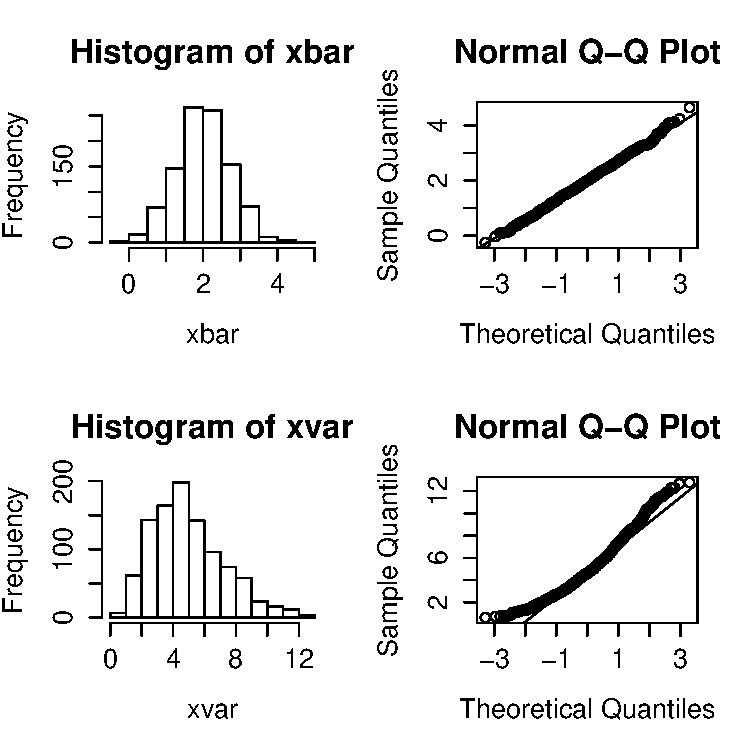
\includegraphics[width=8cm]{simulation}
	\caption{Normal Q-Q plot for case i}
\end{figure}

 All values can be obtained by running the function with the values given in the question. And by comparing the values from these four sets of runs, we can see the value of coverage is essentially very close to $1-\alpha$ for both $\alpha = 0.05 and 0.025$. The coverage may also increase a little bit when using a larger-size (larger n) model by comparing the runs for the same $\alpha$ but different n values. These observations would be very useful when setting up simulation for certain applications.
 
 \begin{lstlisting}[language=R, breaklines=T, basicstyle=\footnotesize\ttfamily]
 
 > fsample(2,5^0.5,10,1000,0.05)
 sample mean: 2.003523 
 sample variance: 4.949434 
 sample confidence interval: [ 0.617619 , 3.389427 ] 
 coverage: 0.953 
 
 > fsample(2,5^0.5,10,1000,0.025)
 sample mean: 2.003523 
 sample variance: 4.949434 
 sample confidence interval: [ 0.4186117 , 3.588434 ] 
 coverage: 0.973 
 
 > fsample(2,5^0.5,100,1000,0.05)
 sample mean: 1.998911 
 sample variance: 5.014552 
 sample confidence interval: [ 1.560649 , 2.437172 ] 
 coverage: 0.958 
 
 > fsample(2,5^0.5,100,1000,0.025)
 sample mean: 1.998911 
 sample variance: 5.014552 
 sample confidence interval: [ 1.497718 , 2.500103 ] 
 coverage: 0.98 
 
 \end{lstlisting}
 
 \paragraph{(c) Simulation with estimated $\sigma^2 $} In the case that $\sigma^2$ is unknown, the sample variance can be estimated by the standard error of the sample. The function is modified by removing $\sigma$ in the calculation and using standard error (via  \textit{sd()} ) to estimate the confidence interval. The modified function is shown below.
 
 \begin{lstlisting}[language=R, breaklines=T, basicstyle=\footnotesize\ttfamily]
 
 fsample<-function(mu,sigma,n,nsim,alpha)
 { xbar<-rep(0,nsim);xvar<-rep(0,nsim); 
 
 # calculate confidence interval
 
 xpred_lower_estimate <- rep(0, nsim)
 xpred_upper_estimate <- rep(0, nsim)
 s <- rep(0, nsim)
 
 for(i in 1:nsim)
 {set.seed(i)
 # x contains a random sample of size n of the variable X
 x<-rnorm(n,mu,sigma)
 xbar[i]<-mean(x)
 xvar[i]<-var(x)
 s[i] = sd(x)
 
 # use standard error instead of variance to calucalate lower and upper bound
 
 xpred_lower_estimate[i] = xbar[i] + qnorm(alpha/2) * s[i] / n^0.5;
 xpred_upper_estimate[i] = xbar[i] - qnorm(alpha/2) * s[i] / n^0.5;
 
 }
 
 cat('sample mean:',mean(xbar),"\n")
 cat('estimated sample confidence interval: [', mean(xpred_lower_estimate), ",", mean(xpred_upper_estimate), "] \n")
 cat('esimated coverage:', mean( mu >=  xpred_lower_estimate & mu <= xpred_upper_estimate) )

 }
 

 fsample(2,5^0.5,10,1000,0.05)
 fsample(2,5^0.5,10,1000,0.025)
 fsample(2,5^0.5,100,1000,0.05)
 fsample(2,5^0.5,100,1000,0.025)
 
 
 \end{lstlisting}
 
 The results for all four cases are shown below. They are deviated from the result that we've got from question (b) since in this case the variance has to be estimated. Meanwhile, when a larger-size sample is introduced the coverage in this case is larger and closer to $1-\alpha$. Therefore, when the $\sigma^2$ is unknown and has to be estimated, it would be more fruitful to take a large sample size (n) to get a more decent coverage.
 
\begin{lstlisting}[language=R, breaklines=T, basicstyle=\footnotesize\ttfamily]

> fsample(2,5^0.5,10,1000,0.05)
sample mean: 2.003523 
estimated sample confidence interval: [ 0.6621783 , 3.344867 ] 
esimated coverage: 0.911

> fsample(2,5^0.5,10,1000,0.025)
sample mean: 2.003523 
estimated sample confidence interval: [ 0.4695695 , 3.537476 ] 
esimated coverage: 0.943

> fsample(2,5^0.5,100,1000,0.05)
sample mean: 1.998911 
estimated sample confidence interval: [ 1.561131 , 2.43669 ] 
esimated coverage: 0.955

> fsample(2,5^0.5,100,1000,0.025)
sample mean: 1.998911 
estimated sample confidence interval: [ 1.498269 , 2.499552 ] 
esimated coverage: 0.977

\end{lstlisting}


\section{Posterior distribution}

The likelihood function is given by:
\begin{equation}
L(X|\sigma^2) \propto (\sigma^2)^{-n/2}exp\{-\sum_{i=1}^{n} X_i^{2}/(2\sigma^2)\}
\end{equation}

The prior distribution of $\sigma^2$ is given by:
\begin{equation}
\pi (\sigma^2) \propto (\sigma^2)^{-(\alpha + 1)}exp\{-\beta/\sigma^2\}
\end{equation}

Then the posterior density of $\sigma^2$ is:
\begin{equation}
\begin{aligned}
\pi (\sigma^2| X_1, X_2, ..., X_n)  \propto \\ (\sigma^2)^{-n/2-(\alpha + 1)}exp\{-\sum_{i=1}^{n} X_i^{2}/(2\sigma^2)-\beta/\sigma^2\}
\begin{aligned}
\end{equation}

Which is equivalent to:
\begin{equation}
\begin{aligned}
	\pi (\sigma^2| X_1, X_2, ..., X_n)  \propto \\ (\sigma^2)^{-(n/2 + \alpha + 1)}exp\{-((\sum_{i=1}^{n} X_i^{2})/2 + \beta)/\sigma^2\}
\end{aligned}
\end{equation}


By comparing the equation obtained with the pdfs of some common distributions, it is concluded that $\sigma^2 $ looks like an  Invgamma ($ n/2 + \alpha, (\sum_{i=1}^{n} X_i^{2})/2 + \beta) $) distribution. 

\section{Rejection method}

\paragraph{(a)} 
\subparagraph{Construct an algorithm}Figure 2 shows a comparison of random sample (x) proposed algorithm and actual Beta random sample (X0). The Beta random sample was constructed by generating two sets of Gamma random variables (via \textit{rgamma()}) following the algorithm. Meanwhile, the actual Beta random sample was generated by \textit{rbeta()}. The parameters were set at $\alpha = 2$ and $\beta = 2$. The sample size was set at 10000. 
\begin{lstlisting}[language=R, breaklines=T, basicstyle=\footnotesize\ttfamily]

fbeta <- function (n, alpha, beta)
{
x1 <- rgamma(n ,shape = alpha, scale = 1)
x2 <- rgamma(n ,shape = beta, scale = 1)
x<- x1/(x1+x2)

x0 <- rbeta(n, alpha, beta, ncp = 0)
# return(x)
par(mfrow=c(2,2))  
hist(x);qqnorm(x);qqline(x);
hist(x0);qqnorm(x0);qqline(x0);

}

fbeta(10000, 2, 2)

\end{lstlisting}

\subparagraph{Density histogram }It can be seen from Figure 2 that the proposed algorithm can match the beta distribution very well. And the Q-Q plot looks reasonable except at the boundaries.  

\begin{figure}
	\centering 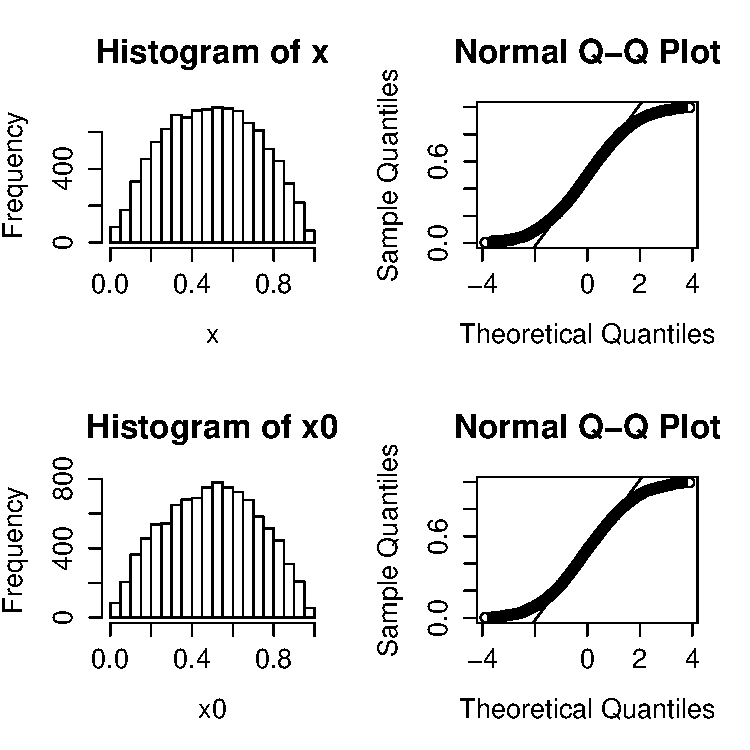
\includegraphics[width=8cm]{beta1}
	\caption{Normal Q-Q plot for case i}
\end{figure}


\paragraph{(b) Rejection method} 

\subparagraph{(i) Uniform distribution}
When $\alpha = 2$ and $\beta = 2$, the pdf of beta distribution can be written as: 


\begin{equation}
f (x) = 6x(1-x)
\end{equation}

The uniform distribution can be written as:

\begin{equation}
\begin{aligned}
g_1 (x) = 1
\end{aligned}
\end{equation}
From the pdfs mentioned above, we were able to calculate the value of c1 according to the equation below:
\begin{equation}
\begin{aligned}
c = max((f(y)/g(y))
\end{aligned}
\end{equation}

Considering the first and second derivatives of $f(y)/g_1(y)$, the value of c1 can be calculated. The rejection sampling was then repeated by a for loop in R until a sufficient number of accepted x's were obtained.

\begin{equation}
\begin{aligned}
c1 = max((f(y)/g_1(y)) = max(6x(1-x)) \\= 1.5
\end{aligned}
\end{equation}

\begin{lstlisting}[language=R, breaklines=T, basicstyle=\footnotesize\ttfamily]
# choose uniform distribution as proposed function
for(i in 1: (10000*c1))
{
u = runif(1)
y = runif(1)
if( u <=  dbeta(y, alpha, beta)/(dunif(1)*c1)) 
{ x = c(x,y)}
}
\end{lstlisting}
Figure 3 shows the density histograms constructed for (i) uniform distribution. In this case a large sample size (10000) was used and the result (i) are pretty close to the histogram obtained in question (a). In addition, the mean value of accepted values equals to 1/c, which agrees with the theory of rejection method.

\begin{figure}
	\centering \includegraphics[width=8cm]{unif}
	\caption{Normal Q-Q plot for (i) uniform distribution}
\end{figure}


\subparagraph{(ii) Truncated distribution}
The truncated normal distribution can be written as:

\begin{equation}
\begin{aligned}
g_2 (x) = \phi(x) /(\Phi (1)- \Phi(0))
\end{aligned}
\end{equation}

From the pdfs mentioned above, we were able to calculate the value of c2 according to the equation below:

\begin{equation}
\begin{aligned}
c = max((f(y)/g(y))
\end{aligned}
\end{equation}

Considering the first and second derivatives of  $f(y)/g_2(y)$, the value of c2 can be calculated. The rejection sampling was then repeated by a for loop in R until a sufficient number of accepted x's were obtained.

\begin{equation}
\begin{aligned}
c2 = max((f(y)/g_2(y))\\ = max(6x(1-x)/(\phi(x) /(\Phi (1)- \Phi(0)))) \\= 4.34
\end{aligned}
\end{equation}

\begin{lstlisting}[language=R, breaklines=T, basicstyle=\footnotesize\ttfamily]
# choose truncated normal distribution as proposed function
for(i in 1: (10000*c2))
{
u = runif(1)
y = rtruncnorm(1, a= 0, b= 1, mean = 1, sd = 2)
if( u <=  dbeta(y, alpha, beta)/(dtruncnorm(y, a = 0, b = 1, mean = 0, sd =1)*c2)) 
{ x = c(x,y)}
}
\end{lstlisting}

Figure 4 shows the density histograms constructed for (ii) truncated normal distribution. In all the cases a large sample size (10000) was used and the result for both (i) and (ii) are pretty close to the histogram obtained in question (a). In addition, the mean value of accepted values equals to 1/c, which agrees with the theory of rejection method.

\begin{figure}
	\centering 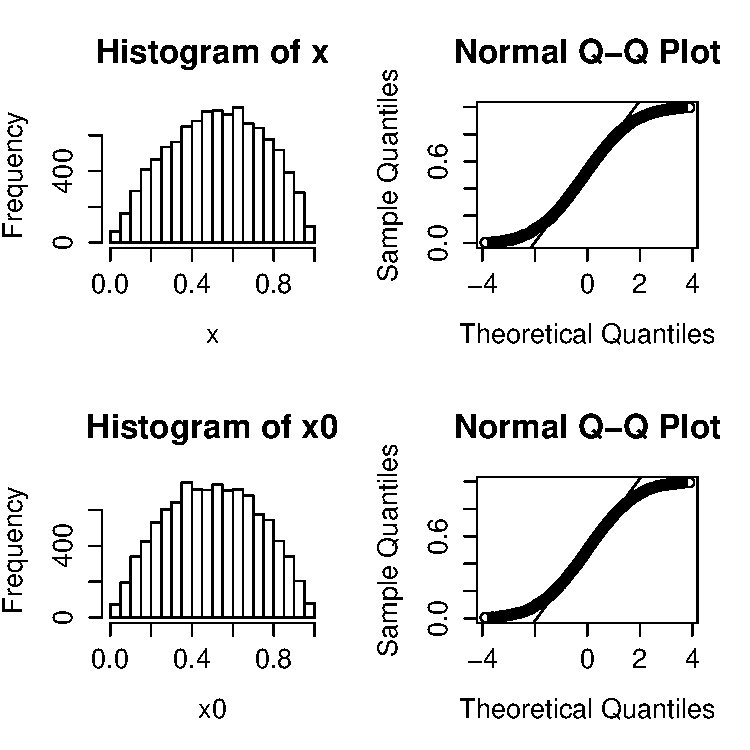
\includegraphics[width=8cm]{truncated}
	\caption{Normal Q-Q plot for (ii) truncated normal distribution}
\end{figure}


\section{Monte Carlo Integration}

\paragraph{(a) MC integration for estimating $\theta$}Since 
\begin{equation}
\begin{aligned}
\theta = \int_{0}^{\infty} exp (-(\sqrt{x}+0.5x))\sin^2(x) dx  \\ = \int_{0}^{\infty} h(x) f(x) dx 
\end{aligned}
\end{equation}

It is obvious that 

\begin{equation}
\begin{aligned}
h(x) = exp (-(\sqrt{x}+0.5x))\sin^2(x) / f(x) \\ = exp (-(\sqrt{x}+0.5x))\sin^2(x)/ (0.5 exp(-0.5x)) \\ = 2 sin^2(x) exp(-\sqrt{x})
\end{aligned}
\end{equation}

Monte Carlo (MC) integration draws a large number of $x_1, x_2, ..., x_n $ of random variables from f(x) which follows exponential distribution with $\lambda = 0.5 $, then

\begin{equation}
\theta \simeq (1/n)\sum_{n=1}^{n} h(x_i)
\end{equation}

Both $f(x)$ and $h(x)$ are already known, so the value of $\theta$ can be obtained depending on different value of $n$. Here we can define a new function integral to calculate the integral from $h(x)$, as shown below:

\begin{lstlisting}[language=R, breaklines=T, basicstyle=\footnotesize\ttfamily]
integral = function (n){
x = rexp(n, rate = 0.5)
# evaluate the mean with different n, show the figure of mean vs n
hx = 2 * (sin(x)^2)*exp(-x^0.5)
theta = mean(hx)
return (theta)
}
\end{lstlisting}
When n = 10000, the theta is 0.2624. And a large number of n is recommended (Figure 5 reveals how the sample size affect the integral, the integral starts to converge after a certain value of n). Additionally, the integral can be directly calculated from a R build-in function integrate(), and the calculated value is 0.2617744 with absolute error $<$ 1.6e-05. So the result from MC integration is very close to actual value.

\begin{figure}[h]
	\centering 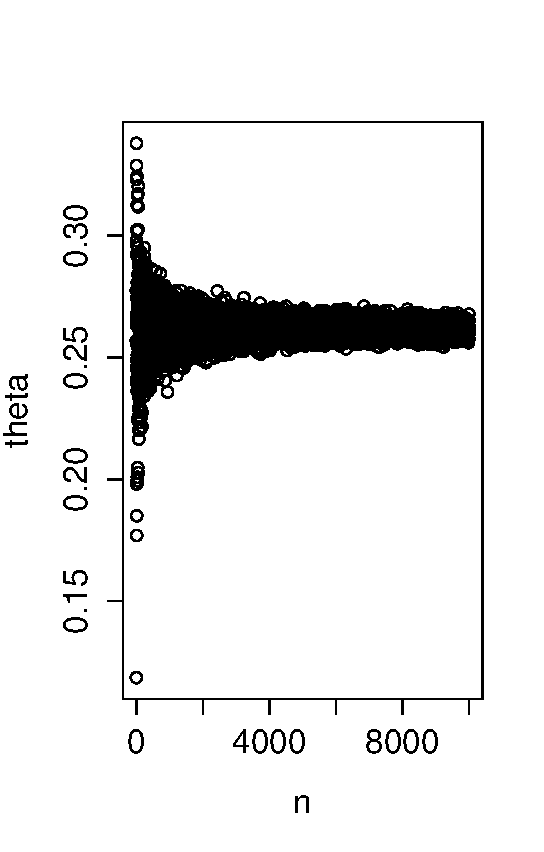
\includegraphics[width=8cm]{theta}
	\caption{Choose the proper sample size when doing MC integration}
\end{figure}

\paragraph{(b) Importance sampling} It can be seen that $g_1(x)$ follows a Laplace distribution with $\mu = 0$ and $b = 1$; $g_2(x)$ follows a Cauchy distribution with $x_0 = 0$ and $\gamma = 2 $; and $g_3(x)$ follows a normal distribution with $\mu = 0$ and $\sigma = 1$.
And the each function, we derive the $f(x)h(x)/g(x)$:
For  $g_1(x)$: 
\begin{equation}
\begin{aligned}
f(x)h(x)/g(x) \\= 2(sin(x))^2  exp (-x^{0.5} - 0.5x + |x|)
\end{aligned}
\end{equation}

For  $g_2(x)$: 
\begin{equation}
\begin{aligned}
f(x)h(x)/g(x) \\ = 2\pi(1+(x^2/4)) (sin(x))^2  exp (-x^{0.5} - 0.5x)
\end{aligned}
\end{equation}

For  $g_3(x)$: 
\begin{equation}
\begin{aligned}
f(x)h(x)/g(x) \\ = (2\pi)^{0.5}  exp(x^2/2) (sin(x))^2  exp (-x^{0.5} - 0.5x)
\end{aligned}
\end{equation}

The means and standard deviations of the estimates when M = 100, 500, 1000, 2000 are given below. Overall, when using $g_2(x)$ and $g_3(x)$ the final results are close to the value we got from question (a). And the results from $g_1(x)$ are still reasonable but not so close to the truth. When using a larger sample size we get a higher chance to get an estimate which is close to the truth and the standard deviation will get much smaller when using a large sample size like 1000 and 2000. These different values of mean and standard deviations provide insight into the design of a good importance sampling. It is very critical to know that the choice of $g(x)$ may have a direct effect on the performance of MC integration.

\begin{lstlisting}[language=R, breaklines=T, basicstyle=\tiny]
M = 100
              [mean]       [sd]      [lb]      [up]
        g1 0.3411303 0.04235505 0.2581159 0.4241446
        g2 0.2587114 0.04358765 0.1732812 0.3441416
        g3 0.2438155 0.04125228 0.1629625 0.3246685
M = 500        
        g1 0.2903797 0.01926343 0.2526241 0.3281353
        g2 0.2842341 0.02115650 0.2427681 0.3257001
        g3 0.2453785 0.01679555 0.2124599 0.2782972
M = 1000		
        g1 0.3110603 0.01310886 0.2853674 0.3367532
        g2 0.2569927 0.01391424 0.2297213 0.2842641
        g3 0.2589525 0.01239662 0.2346555 0.2832494
M = 2000
        g1 0.3179534 0.009634396 0.2990704 0.3368365
        g2 0.2502560 0.009578289 0.2314829 0.2690292
        g3 0.2365543 0.011748052 0.2135285 0.2595800
\end{lstlisting}


\paragraph{(c) Self-normalized importance sampling} To choose a good importance sampling distribution requires some educated
guessing and possibly numerical search. Figure 6 shows the actual plots for target function (via wolframalpha) The self-normalized importance sampler requires a stronger condition than the unbiased importance sampler does. The optimal density for self-normalized importance sampling has the form $g(x) \propto |f(x)-\mu|h(x)$.

Here we consider a probability function that is a linear combination of multiple normal distributions with mean = $\pi/2, 3\pi/2, 5\pi/2, ... (2n-1)\pi/2.$ To demonstrate the idea we take the first three terms to draw sample from the following distribution to make sure it is as close to $|f(x)-\mu|h(x)$ as possible:

$$ 0.5 N(\pi/2) + 0.3 N(3\pi/2) + 0.2 N(5\pi/2) $$

As shown in the code below. The weight for each density function was set at 0.5, 0.3 and 0.2 receptively because the plot has more area under the first peak (corresponding to the first density function).

\begin{lstlisting}[language=R, breaklines=T, basicstyle=\footnotesize\ttfamily]

# draw samples from a mixture of three normal distributions with mean = (pi/2,3*pi/2,5*pi/2) weight = (0.5,0.3,0.2) and variance = sqrt(c(1,1,1)).
N <- 2000

components <- sample(1:3,prob=c(0.5,0.3,0.2),size=N,replace=TRUE)
mus <- c(pi/2,3*pi/2,5*pi/2)
sds <- sqrt(c(1,1,1))

X <- rnorm(n=N,mean=mus[components],sd=sds[components])
\end{lstlisting}

\begin{figure}
	\centering 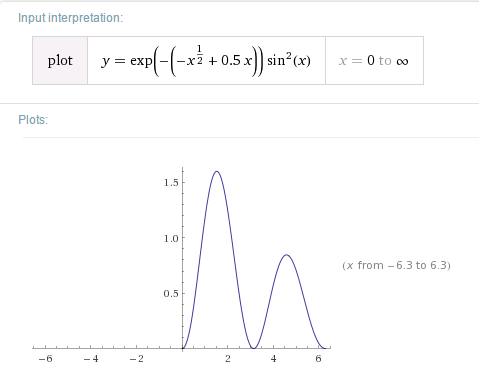
\includegraphics[width=8cm]{function}
	\caption{Plot of target function for integration}
\end{figure}
By using the same method as in question(b), we were able to integrate the target function using random variables drawing from the new proposed function. And the result of integration is shown below:

\begin{lstlisting}[language=R, breaklines=T, basicstyle=\footnotesize\ttfamily]
M = 100
   [mean]       [sd]      [lb]      [up]
0.260415280 0.000729035 0.258986398 0.261844162
\end{lstlisting}
The obtained mean value (0.26) is almost the same as the truth. Thus it is clear that with a better information of target function and self-normalized importance sampling, the integration will be more optimized. And in reality it is hard to get an exact optimized expression $g(x)$, but it would be helpful to choose $g(x)$ such that the estimator obtained by importance sampling has finite variance.

\end{document}
